\begin{examplebox}

    \textbf{\textcolor{CExample}{例零（初中衔接：先学会选一条方便的底边）}}

    \textbf{题目：}已知 $A(0,2)$、$B(4,6)$、$P(2,0)$，$M$ 为 $AB$ 中点，
    不求 $AB$ 的长度，求 $S_{\triangle PAB}$。

    % 初中衔接：精确坐标 A(0,2), B(4,6), P(2,0), M(2,4)
\begin{center}
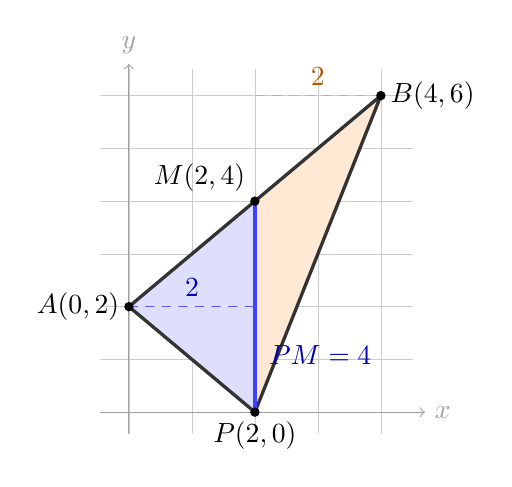
\begin{tikzpicture}[x=0.8cm,y=0.67cm, line cap=round, line join=round]
  \draw[gray!40,step=1,very thin] (-0.45,-0.4) grid (4.5,6.5);
  \draw[->,gray!75] (-0.45,0)--(4.7,0) node[right] {$x$};
  \draw[->,gray!75] (0,-0.4)--(0,6.6) node[above] {$y$};
  \coordinate (A) at (0,2);
  \coordinate (B) at (4,6);
  \coordinate (P) at (2,0);
  \coordinate (M) at (2,4);
  \fill[blue!13] (P)--(A)--(M)--cycle;
  \fill[orange!17] (P)--(M)--(B)--cycle;
  \draw[very thick,black!80] (P)--(A)--(B)--cycle;
  \draw[very thick,blue!75] (P)--(M);
  \draw[dashed,blue!65] (A)--(0,2)--(2,2);
  \draw[dashed,orange!75] (B)--(2,6);
  \fill (A) circle (1.7pt) node[left] {$A(0,2)$};
  \fill (B) circle (1.7pt) node[right] {$B(4,6)$};
  \fill (P) circle (1.7pt) node[below] {$P(2,0)$};
  \fill (M) circle (1.7pt) node[above left] {$M(2,4)$};
  \node[blue!70!black,anchor=south] at (1,2.0) {$2$};
  \node[orange!70!black,anchor=south] at (3.0,6.0) {$2$};
  \node[blue!70!black,right] at (2.07,1.08) {$PM=4$};
\end{tikzpicture}
\end{center}


    \textbf{第一步（中点）：}
    $M\left((0+4)/2,(2+6)/2\right)=(2,4)$，
    所以 $PM$ 是竖直线段，$PM=4$。

    \textbf{第二步（两侧的水平高）：}
    $h_A=|0-2|=2$，$h_B=|4-2|=2$。

    \textbf{第三步（分块面积）：}
    \[
       S_{\triangle PAB}
       =\frac12\cdot4\cdot2+\frac12\cdot4\cdot2
       =\boxed{8}.
    \]
    \textbf{迁移：}这一题不涉及抛物线，但已经用到了 C072 里
    \textbf{最关键的面积思路}：先找竖直中线，再用水平距离作高。

    \medskip

    \par\noindent\begin{minipage}{\linewidth}
    \textbf{\textcolor{CExample}{例一（基础：顶点、中线与面积一起求）}}

    \textbf{题目：}抛物线 $x^2=4y$ 上有 $A(2,1)$、$B(4,4)$，
    两切线交于 $P$，$M$ 为 $AB$ 中点。求 $P,M,PM$ 及 $S_{\triangle PAB}$。

    \end{minipage}\par
    \textbf{第一步（核对曲线与参数）：} $x^2=4y=2py$，故 $p=2$。
    $2^2=4\times1$、$4^2=4\times4$，两点均在曲线上。

    \textbf{第二步（交点与中点）：}
    \[
        P\left(\frac{2+4}{2},\frac{2\times4}{2\times2}\right)=(3,2),
        \quad M\left(\frac{2+4}{2},\frac{1+4}{2}\right)
        =\left(3,\frac52\right).
    \]
    因两点横坐标都为 $3$，所以 $PM$ 竖直，
    \[
        PM=\frac52-2=\frac12.
    \]

    \textbf{第三步（不用点线距离就求面积）：}
    以 $PM$ 为底，左右两侧的水平高分别为 $|2-3|=1$ 和 $|4-3|=1$，
    \[
        S=\frac12\times\frac12\times1
          +\frac12\times\frac12\times1=\boxed{\frac12}.
    \]
    用公式核对：$|2-4|^3/(8\times2)=8/16=1/2$。
    \textbf{提醒：}这里 $AB$ 的斜率为 $(4-1)/(4-2)=3/2$，
    故竖直的 $PM$ 并不垂直 $AB$，不能把它说成“$AB$ 上的高”。

    \medskip
    \textbf{\textcolor{CExample}{例二（逆向：已知面积求水平距离）}}

    \textbf{题目：}在 $x^2=2y$（$p=1$）中，某两切线三角形面积为 $1$。
    求 $|x_1-x_2|$。

    \textbf{第一步（把条件代入面积公式）：}
    \[
        1=\frac{|x_1-x_2|^3}{8\times1}
        \quad\Longrightarrow\quad |x_1-x_2|^3=8.
    \]
    \textbf{第二步（开立方）：} 因 $|x_1-x_2|>0$，
    \[
        \boxed{|x_1-x_2|=2}.
    \]
    \textbf{容易忽略的地方：}只能得到\textbf{两横坐标之差的绝对值}，
    不能据此断定两个切点就是 $x_1=-1,x_2=1$。
    例如 $(x_1,x_2)=(0,2)$ 也满足此条件。

    \medskip
    \textbf{\textcolor{CExample}{例三（综合：给出两切线交点求面积）}}

    \textbf{题目：}从 $Q(4,1)$ 向抛物线 $x^2=4y$ 作两条切线，
    切点为 $A,B$，求 $S_{\triangle QAB}$。

    \textbf{第一步（先核对确有两条切线）：}
    此处 $p=2$、$(x_0,y_0)=(4,1)$，
    \[
        x_0^2-2py_0=4^2-2\times2\times1=12>0.
    \]
    所以存在两个不同的实切点。

    \textbf{第二步（反求两个切点的横坐标）：}
    \[
        x^2-2x_0x+2py_0=0
        \quad\Longrightarrow\quad x^2-8x+4=0.
    \]
    用配方法：
    \[
        (x-4)^2=12
        \quad\Longrightarrow\quad
        x_1=4-2\sqrt3,\quad x_2=4+2\sqrt3.
    \]
    所以
    \[
        |x_1-x_2|=4\sqrt3.
    \]

    \textbf{第三步（计算面积）：}
    \[
    \begin{aligned}
        S_{\triangle QAB}
        &=\frac{(4\sqrt3)^3}{8\times2}\\
        &=\frac{64\times3\sqrt3}{16}
         =\boxed{12\sqrt3}.
    \end{aligned}
    \]
    \textbf{更快的核对：}
    $S=(x_0^2-2py_0)\sqrt{x_0^2-2py_0}/p
    =12\sqrt{12}/2=12\sqrt3$。

    \medskip
    \textbf{\textcolor{CExample}{例四（迁移：开口方向互换）}}

    \textbf{题目：}抛物线 $y^2=4x$ 上有 $A(1,2)$、$B(4,4)$，
    两切线交于 $P$，求 $P$ 与三角形面积。


    \begin{center}
\begin{tikzpicture}[x=.9cm,y=.9cm,font=\small,>=Stealth]
\foreach \shift/\swap/\title in {0/0/{$x^2=4y$：竖直中线},7/1/{$y^2=4x$：水平中线}} {
\begin{scope}[xshift=\shift cm]
\node[anchor=south] at (2,5) {\title};
\draw[->,gray] (-.4,0)--(4.9,0) node[right] {$x$};
\draw[->,gray] (0,-.4)--(0,4.7) node[above] {$y$};
\ifnum\swap=0
\coordinate (A) at (2,1); \coordinate (B) at (4,4);
\coordinate (P) at (3,2); \coordinate (M) at (3,2.5);
\draw[blue!70!black,thick,domain=0:4.2,samples=70] plot (\x,{\x*\x/4});
\node at (3.5,1.8) {$P$}; \node at (2.5,2.7) {$M$};
\else
\coordinate (A) at (1,2); \coordinate (B) at (4,4);
\coordinate (P) at (2,3); \coordinate (M) at (2.5,3);
\draw[blue!70!black,thick,domain=0:4.2,samples=70] plot ({\x*\x/4},\x);
\node at (1.6,3.4) {$P$}; \node at (2.8,2.7) {$M$};
\fi
\fill[blue!12] (P)--(A)--(B)--cycle;
\draw[thick] (P)--(A)--(B)--cycle;
\draw[orange!80!black,very thick] (P)--(M);
\foreach \pt/\pos in {A/below right,B/above left}
  \fill (\pt) circle (1.5pt) node[\pos] {$\pt$};
\fill (P) circle (1.5pt); \fill (M) circle (1.5pt);
\end{scope}}
\end{tikzpicture}
\end{center}


    \textbf{第一步（明确不能直接照抄）：}
    $y^2=4x$ 的对称轴是 $x$ 轴，不是 $y$ 轴。
    在公式中将 $x,y$ 互换，且仍有 $p=2$，得到
    \[
        P\left(\frac{y_1y_2}{2p},\frac{y_1+y_2}{2}\right)
        =\left(\frac{2\times4}{4},\frac{2+4}{2}\right)=(2,3).
    \]

    \textbf{第二步（把水平与竖直的角色互换）：}
    $AB$ 中点 $M=((1+4)/2,(2+4)/2)=(5/2,3)$，
    故 $PM$ 水平，$PM=1/2$；两个切点的竖直距离是 $|4-2|=2$。
    \[
        S=\frac12\times PM\times|y_2-y_1|
        =\frac12\times\frac12\times2=\boxed{\frac12}.
    \]
    用互换后的面积公式核对：$|y_1-y_2|^3/(8p)=8/16=1/2$。
    \textbf{迁移信号：}抛物线方向互换时，凡涉及“横坐标差”“竖直中线”
    的叙述，都要对应换成“纵坐标差”“水平中线”。
\end{examplebox}
